\documentclass[12pt,a4paper]{article}

% ── Packages ────────────────────────────────────────────────────────────────
\usepackage[T1]{fontenc}
\usepackage[utf8]{inputenc}
\usepackage[margin=2.5cm]{geometry}
\usepackage{booktabs}
\usepackage{tabularx}
\usepackage{hyperref}
\usepackage{setspace}
\usepackage{titlesec}
\usepackage{fancyhdr}
\usepackage{float}
\usepackage{enumitem}
\usepackage{xcolor}
\usepackage{tikz}
\usetikzlibrary{shapes.geometric, arrows.meta, positioning, fit, backgrounds}
\usepackage{amsmath}
\usepackage{parskip}
\usepackage{abstract}

% ── Typography ───────────────────────────────────────────────────────────────
\onehalfspacing
\setlength{\parskip}{6pt}

% ── Section formatting ───────────────────────────────────────────────────────
\titleformat{\section}{\large\bfseries}{{\thesection}}{1em}{}[\titlerule]
\titleformat{\subsection}{\normalsize\bfseries}{\thesubsection}{1em}{}
\titleformat{\subsubsection}{\normalsize\itshape}{\thesubsubsection}{1em}{}

% ── Header / Footer ──────────────────────────────────────────────────────────
\pagestyle{fancy}
\fancyhf{}
\rhead{\small Egyptian Pharmacy AI Subagent}
\lhead{\small Graduation Project Report}
\cfoot{\thepage}
\renewcommand{\headrulewidth}{0.4pt}

% ── TikZ styles ──────────────────────────────────────────────────────────────
\tikzstyle{block} = [rectangle, rounded corners=4pt, minimum width=3.4cm,
    minimum height=0.9cm, text centered, draw=black, fill=blue!8, font=\small]
\tikzstyle{safeblock} = [rectangle, rounded corners=4pt, minimum width=3.4cm,
    minimum height=0.9cm, text centered, draw=black, fill=red!10, font=\small]
\tikzstyle{llmblock} = [rectangle, rounded corners=4pt, minimum width=3.4cm,
    minimum height=0.9cm, text centered, draw=black, fill=green!10, font=\small]
\tikzstyle{arrow} = [thick,->,>=Stealth]

% ── Hyperref ─────────────────────────────────────────────────────────────────
\hypersetup{colorlinks=true, linkcolor=black, urlcolor=blue!60!black, citecolor=black}

% ─────────────────────────────────────────────────────────────────────────────
\begin{document}

% ── Title page ───────────────────────────────────────────────────────────────
\begin{titlepage}
    \centering
    \vspace*{2cm}
    {\LARGE\bfseries Egyptian Pharmacy AI Subagent\par}
    \vspace{0.5cm}
    {\large A Retrieval-Augmented Medication Guidance System\par}
    \vspace{1.5cm}
    \rule{0.6\textwidth}{0.4pt}\\[1em]
    {\large Graduation Project Report\par}
    \vspace{0.5cm}
    {\normalsize June 2026\par}
    \vspace{2cm}
    \begin{abstract}
        \noindent
        This report presents the design, methodology, and evaluation of a
        pharmacy-focused AI subagent built for the Egyptian drug market.
        The system addresses a concrete gap in digital healthcare: patients
        seeking medication guidance are frequently exposed to inaccurate
        information, including hallucinated drug names and prices produced
        by general-purpose language models unaware of the Egyptian drug
        registry. The proposed system combines a curated pharmaceutical
        dataset, a three-channel hybrid retrieval pipeline, a clinical
        safety screening layer, and a large language model to deliver
        grounded, hallucination-resistant medication guidance in Egyptian
        Arabic. Designed as a specialised subagent within a broader
        voice-agent healthcare workflow, the system strictly confines
        itself to pharmacy tasks and escalates all out-of-scope requests
        to the primary orchestrator.
    \end{abstract}
    \vfill
    {\small\textit{Graduation Project --- June 2026}}
\end{titlepage}

% ── Table of contents ────────────────────────────────────────────────────────
\tableofcontents
\newpage

% ─────────────────────────────────────────────────────────────────────────────
\section{Introduction}

\subsection{Motivation}

Access to accurate medication information is a significant challenge in Egypt.
Patients and caregivers routinely seek guidance for self-limiting conditions
and over-the-counter (OTC) purchases, yet the advice available to them is
inconsistent in accuracy, lacks price transparency, and is rarely tailored
to individual contraindications or allergy profiles.

The rise of general-purpose AI assistants has not resolved this problem ---
it has compounded it. Large language models trained on broad internet corpora
can produce confident, fluent responses to medication queries, but they
frequently hallucinate drug names, invent prices, and reference products
that are not registered in the Egyptian market. A patient acting on such
a response risks purchasing a non-existent product, taking an unsafe dose,
or missing a contraindication relevant to their health profile.

This project was motivated by the need for a medication guidance system that
is both conversationally capable and factually grounded --- one that draws
every drug name, price, and clinical warning directly from a verified
Egyptian pharmaceutical dataset rather than from a language model's
parametric memory.

\subsection{Problem Statement}

The core problem addressed by this project is the lack of a reliable medication
assistant tailored to the Egyptian pharmaceutical market. General-purpose AI
systems may provide medication-related information, but they are not grounded
in local drug data and may generate inaccurate or unsupported responses.

This project aims to provide a pharmacy-focused assistant that delivers accurate
drug information, prices, active ingredients, and substitute recommendations
based on a curated Egyptian medication dataset. The system follows a
retrieval-first approach, ensuring that medication information originates from
verified dataset records rather than model-generated content.

In addition, the assistant is intentionally limited to pharmacy-related tasks.
It does not perform medical diagnosis, treatment planning, appointment booking,
or emergency triage. Requests that fall outside the pharmacy domain are
delegated to the main healthcare orchestrator, ensuring clear separation of
responsibilities and safer user interactions.

\subsection{Design Philosophy}

The system was designed as a specialized pharmacy assistant focused on
medication-related queries. Instead of relying on a large language model as
the primary source of information, the architecture follows a retrieval-first
approach where medication data is retrieved from a curated Egyptian drug
dataset before any response is generated.

This design was chosen to improve reliability when handling medication names,
active ingredients, prices, and substitute recommendations. By separating
information retrieval from response generation, the system reduces the risk
of hallucinated drug information and ensures that pharmaceutical facts
originate from structured dataset records.

The language model is therefore used as a supporting component for
conversational guidance and response formulation, while medication information
remains grounded in the retrieval layer.

\subsection{Why Retrieval-Augmented Generation}

A pure language model approach was evaluated and rejected at the design stage.
Table~\ref{tab:rag-rationale} summarises the key limitations of standalone
LLMs and how Retrieval-Augmented Generation (RAG) addresses each.

\begin{table}[H]
\centering
\caption{Rationale for RAG over a standalone LLM}
\label{tab:rag-rationale}
\renewcommand{\arraystretch}{1.3}
\begin{tabularx}{\textwidth}{>{\bfseries}p{3.8cm} X}
\toprule
LLM Limitation & How RAG Addresses It \\
\midrule
Drug-name hallucination &
    Retrieval is performed against a verified dataset; the LLM is
    prohibited from writing drug names in its output. \\
No Egyptian market knowledge &
    The dataset contains only drugs registered in Egypt, with Arabic
    trade names and EGP prices. \\
No price accuracy &
    Prices are retrieved from the dataset on every query, not generated
    by the model. \\
No auditability &
    Every drug fact is tied to a specific dataset record. \\
Unsafe safety enforcement &
    Contraindication checks require structured drug facts that only
    retrieval can supply; model judgment is insufficient. \\
\bottomrule
\end{tabularx}
\end{table}

RAG separates \emph{factual grounding} (retrieval from the verified dataset)
from \emph{language generation} (conversational explanation by the model).
The model's role is strictly to produce natural-language usage guidance
around facts that have already been retrieved and safety-checked.

% ─────────────────────────────────────────────────────────────────────────────
\section{Dataset Preparation}

\subsection{Dataset Collection}

The pharmaceutical dataset was collected through web scraping from
\href{https://egyptdwa.com/}{EgyptDwa}, a publicly accessible Egyptian drug
information portal that provides medication information available in the
Egyptian market.

The collected records include medication trade names (Arabic and English),
active ingredients, dosage forms, manufacturers, package information, and
listed retail prices. Following the data collection phase, the dataset
underwent several preprocessing steps, including data cleaning, normalisation,
duplicate handling, and price correction, to improve data quality and
consistency.

The resulting dataset serves as the primary knowledge source for the retrieval
system. All medication information presented by the pharmacy assistant is
retrieved from this curated dataset rather than generated directly by the
language model, ensuring greater factual consistency and reducing the risk of
hallucinated drug information.

\subsection{Data Cleaning and Normalisation}

Raw scraped data required a structured cleaning pipeline before use in
retrieval. The key stages were:

\begin{itemize}[leftmargin=1.5em]
    \item \textbf{Missing value handling} --- Records lacking a trade name,
          active ingredient, or dosage form were removed or enriched from
          secondary sources. Fields critical to retrieval and safety
          screening were treated as required.

    \item \textbf{Duplicate removal} --- Exact and near-duplicate records
          were identified and eliminated. Near-duplicate detection addressed
          entries differing only in whitespace, punctuation, or Arabic
          orthographic variation, including Hamza normalisation, Taa
          Marbouta, and Alef Maqsoura equivalences.

    \item \textbf{Active-ingredient normalisation} --- Ingredient strings
          were resolved to canonical International Non-proprietary Names
          (INNs). Common synonyms --- such as \textit{acetaminophen}
          to \textit{paracetamol} --- were unified, and compound
          ingredients were parsed into component tokens to support
          ingredient-level safety screening.

    \item \textbf{Dosage normalisation} --- Numeric strength and unit
          were standardised and extracted into dedicated fields, enabling
          constraint-based numeric matching during retrieval.

    \item \textbf{Bilingual name normalisation} --- Arabic names were
          normalised for common script variants; English names were
          lowercased and stripped of trailing form noise to improve
          matching consistency.

    \item \textbf{Ingredient alias mapping} --- A curated synonym dictionary
          maps colloquial, regional, and alternative spellings to canonical
          INNs, so that queries using brand names or informal names resolve
          correctly to the underlying active ingredient.
\end{itemize}

\subsection{Price Validation and Correction}

Some records scraped from \texttt{egyptdwa.com} contained anomalous or
unrealistic price values, including zero-value entries, implausibly low
figures, and extreme outliers attributable to data-entry errors. A
dedicated price validation and correction stage was introduced to address
these issues before the dataset was used for retrieval.

The correction methodology groups similar medications by shared attributes:
normalised active ingredient, dosage form, strength, and brand prefix.
Within each peer group, the median price serves as the reference value ---
a statistically robust measure resistant to extreme outliers. Entries
deviating substantially from their peer-group median are assigned a
corrected price derived from that median. The original scraped price
is retained alongside the corrected value in every record, preserving
full auditability.

Table~\ref{tab:price-correction} illustrates the scale of corrections
applied to a representative sample of affected records.

\begin{table}[H]
\centering
\caption{Representative price corrections applied by the validation framework}
\label{tab:price-correction}
\renewcommand{\arraystretch}{1.3}
\begin{tabular}{llrrr}
\toprule
Drug & Active Ingredient & Before (EGP) & After (EGP) & Change \\
\midrule
Immunomide 5\,mg 21 Caps.  & lenalidomide & 6{,}998 & 56{,}702 & $+710\%$ \\
Immunomide 25\,mg 21 Caps. & lenalidomide & 8{,}404 & 56{,}702 & $+575\%$ \\
Otathromb 75\,mg 10 Tabs.  & clopidogrel  & 9       & 48       & $+433\%$ \\
Powerecta 5\,mg 1 Tab.     & vardenafil   & 3       & 30.50    & $+917\%$ \\
\bottomrule
\end{tabular}
\end{table}

% ─────────────────────────────────────────────────────────────────────────────
\section{System Architecture}

\subsection{Overview}

The system is structured as a layered pipeline in which each stage has a
single, well-defined responsibility. Queries enter through a REST API and
pass through query understanding, hybrid retrieval, safety screening, and
response grounding before a structured response is returned to the calling
orchestrator. Figure~\ref{fig:architecture} illustrates the end-to-end flow.

\begin{figure}[H]
\centering
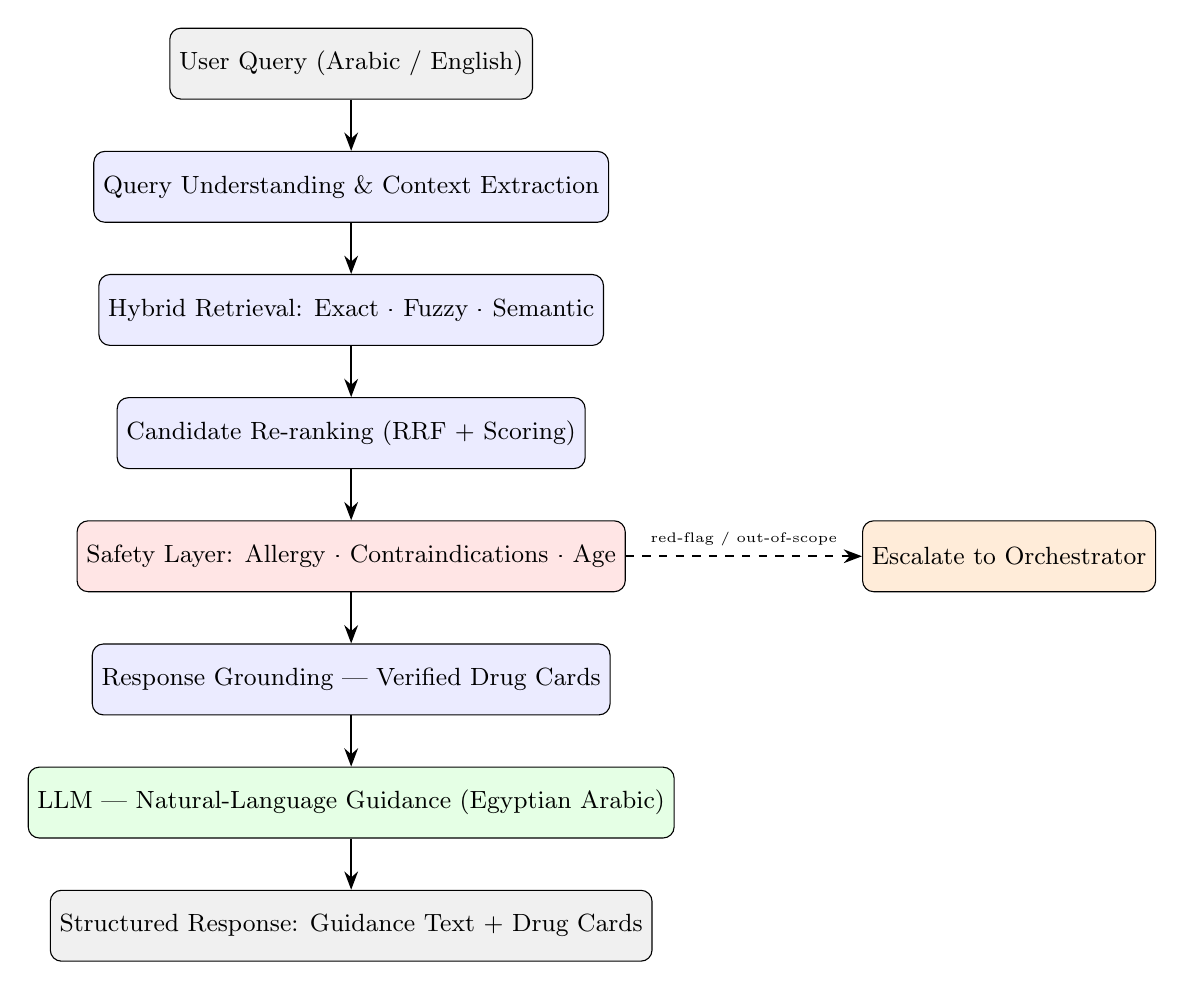
\begin{tikzpicture}[node distance=0.65cm and 0.5cm]

  \node (query)   [block, fill=gray!12]
        {User Query (Arabic / English)};
  \node (context) [block, below=of query]
        {Query Understanding \& Context Extraction};
  \node (hybrid)  [block, below=of context]
        {Hybrid Retrieval: Exact · Fuzzy · Semantic};
  \node (rerank)  [block, below=of hybrid]
        {Candidate Re-ranking (RRF + Scoring)};
  \node (safety)  [safeblock, below=of rerank]
        {Safety Layer: Allergy · Contraindications · Age};
  \node (ground)  [block, below=of safety]
        {Response Grounding --- Verified Drug Cards};
  \node (llm)     [llmblock, below=of ground]
        {LLM --- Natural-Language Guidance (Egyptian Arabic)};
  \node (out)     [block, fill=gray!12, below=of llm]
        {Structured Response: Guidance Text + Drug Cards};

  \foreach \a/\b in {query/context, context/hybrid, hybrid/rerank,
                      rerank/safety, safety/ground, ground/llm, llm/out}
    \draw[arrow] (\a) -- (\b);

  \node (esc) [safeblock, right=3cm of safety, fill=orange!15]
        {Escalate to Orchestrator};
  \draw[arrow, dashed] (safety.east) --
        node[above, font=\tiny]{red-flag / out-of-scope} (esc.west);

\end{tikzpicture}
\caption{End-to-end system pipeline}
\label{fig:architecture}
\end{figure}

\subsection{Main Components}

\begin{description}[leftmargin=0em, style=nextline]

    \item[\textbf{Query Understanding}]
        Each incoming message is parsed to extract a structured patient
        profile covering age, sex, pregnancy and breastfeeding status,
        declared allergens, chronic conditions, current medications, and
        symptom description. The query is simultaneously classified by
        intent: a product information request, a substitute request, or
        an OTC symptom-treatment query. Patient context is accumulated
        across conversation turns so that information declared early in
        the dialogue continues to govern drug selection in later turns.

    \item[\textbf{Hybrid Retrieval Engine}]
        A three-channel retrieval engine searches the pharmaceutical
        dataset using complementary matching strategies. Candidates from
        all channels are merged and re-ranked before safety screening.
        The three channels --- exact matching, fuzzy matching, and
        semantic vector search --- are described in detail in
        Section~\ref{sec:rag}.

    \item[\textbf{Safety Layer}]
        Every candidate drug is screened against the patient's declared
        allergens, chronic conditions, pregnancy or breastfeeding status,
        and age. Contraindicated candidates are suppressed before the LLM
        is invoked. Queries triggering clinical red flags --- such as chest
        pain, severe dyspnoea, or loss of consciousness --- are immediately
        escalated to the orchestrator without drug retrieval.

    \item[\textbf{Response Grounding}]
        Candidates that pass safety screening are assembled into structured
        drug cards drawn directly from dataset fields: Arabic and English
        trade names, active ingredient, dosage form, and price. These
        cards are passed to the LLM as verified context and are also
        returned as structured objects in the API response, independent
        of the model's generated text.

    \item[\textbf{LLM Guidance Layer}]
        The language model receives the patient's message, conversation
        history, patient context, and the pre-assembled drug cards. Its
        role is narrowly defined: produce natural-language usage guidance
        and clinical warnings in colloquial Egyptian Arabic. It is
        explicitly prohibited from writing drug names, prices, or active
        ingredients --- all of which appear only in the structured cards.

    \item[\textbf{Workflow Envelope}]
        Every response includes a structured workflow envelope carrying
        a task status, a flag indicating whether control should return
        to the orchestrator, and an escalation reason where applicable.
        This envelope enables the calling orchestrator to make routing
        decisions without parsing the natural-language text.

\end{description}

\subsection{Data Flow}

A typical OTC query follows this path through the system. The patient's
message and conversation history are received by the API. The query
understanding layer extracts the patient's context and classifies the
intent. The retrieval engine searches the dataset across three channels
and merges the results. The safety layer screens the merged candidates
and suppresses contraindicated drugs. Surviving candidates are assembled
into drug cards, which are passed to the LLM together with the patient
context. The LLM produces guidance text in Egyptian Arabic. The final
response combines the guidance text, the drug cards, and the workflow
envelope, and is returned to the orchestrator.

For product information queries --- where the user asks about a specific
named drug --- the retrieval step targets trade name and active ingredient
fields directly, and no clinical safety gate is applied since the user is
seeking information rather than a recommendation.

% ─────────────────────────────────────────────────────────────────────────────
\section{Retrieval-Augmented Generation Pipeline}
\label{sec:rag}

\subsection{Query Understanding}

Before retrieval begins, the system classifies the query and builds a
patient context record from the full conversation history. Classification
distinguishes three query types: product information requests (questions
about a named drug's price, ingredients, or details), substitute requests
(requests for a therapeutically equivalent alternative), and symptom-based
OTC queries (requests for a drug recommendation based on described symptoms).
Each type activates a different retrieval strategy and different mandatory
safety checks.

Patient context extraction accumulates structured information across turns:
age and sex determine age-gating and pregnancy-check applicability; declared
allergens govern allergy screening; chronic conditions activate
contraindication rules; and red-flag symptom patterns trigger immediate
escalation. Because context is maintained across the conversation, a patient
who mentions a chronic condition early in the dialogue will have that condition
respected for every subsequent drug suggestion.

\subsection{Hybrid Retrieval}

The retrieval engine operates over three complementary channels.

\textbf{Exact name matching} performs deterministic string matching against
the full set of Arabic and English trade names. A match is declared when the
normalised query equals, begins with, or is contained within a normalised drug
name. Exact matches receive a scoring bonus that prevents them from being
displaced by weaker approximate hits.

\textbf{Fuzzy matching} applies an ensemble of five similarity algorithms
(ratio, partial ratio, token sort ratio, token set ratio, and weighted ratio).
The highest score across all five is retained for each candidate, making the
approach more robust than any single algorithm against prefix matches, word
reordering, and partial abbreviations. Separate fuzzy passes target the active
ingredient field, the combined name-plus-ingredient field, and the Arabic and
English name fields independently, each with tuned minimum thresholds.

\textbf{Semantic vector search} performs approximate nearest-neighbour search
over pre-computed multilingual sentence embeddings using a FAISS flat
inner-product index. This channel enables natural-language queries ---
for example, \textit{``something for a blocked nose in children''} --- to
match relevant entries without any token overlap. A multilingual MiniLM
model handles bilingual Arabic/English queries. The embedding index is
built offline and loaded from disk at startup, so only a single short
embedding call per query is required at runtime, keeping memory usage low.

\subsection{Candidate Re-ranking}

Candidates from all three channels are merged into a unified pool.
A Reciprocal Rank Fusion (RRF) mechanism boosts candidates that appear
in more than one channel, proportional to the number of channels that
returned them. The composite scoring function additionally incorporates
ingredient-overlap score, dosage form preference, and numeric strength
compatibility. A relevance gate is applied after re-ranking: substitute
and ingredient-mode queries require strict pharmacological confirmation
before a candidate is passed to the safety layer.

\subsection{Safety Validation}

The safety layer applies four categories of constraint before any drug
is surfaced to the user.

\textbf{Allergy screening} tokenises declared allergens and compares them
at the component level against the active ingredient tokens of every
candidate. A candidate is suppressed if any allergen token matches any
component of its active ingredient string --- an approach that correctly
handles compound ingredients.

\textbf{Contraindication checking} matches the patient's chronic conditions
against a structured knowledge base of ingredient-level contraindication
rules. NSAIDs, for example, are contraindicated in hypertension, kidney
disease, peptic ulcer, and diabetes; decongestants containing
pseudoephedrine are contraindicated in hypertension and heart disease.
Candidates violating any absolute rule are removed from the pool.

\textbf{Pregnancy and breastfeeding restrictions} block NSAIDs, certain
decongestants, and flagged antihistamines for patients who are pregnant
or breastfeeding. When pregnancy status is unknown for a female patient
of childbearing age and the candidate pool contains any flagged ingredient,
the system requests confirmation before proceeding.

\textbf{Age gating} suppresses molecules that carry minimum-age
restrictions for patients who fall below the safe threshold.

\subsection{LLM Guidance Generation and Response Grounding}

Candidates that pass all safety checks are assembled into structured drug
cards containing Arabic and English trade names, active ingredient, dosage
form, and price --- all drawn directly from dataset fields. These cards are
passed to the language model as verified context. The model's system prompt
explicitly instructs it that drug details are displayed in separate cards
and must not be reproduced or paraphrased in the generated text; its sole
task is to produce usage guidance and warnings in colloquial Egyptian Arabic.

As a defence-in-depth measure, a post-processing step scans the model's
output and removes any drug names, prices, or ingredient strings that appear
verbatim, replacing them with neutral phrasing. This ensures that even if
the model violates the system prompt constraint, no hallucinated drug facts
propagate to the final response. The drug cards are returned to the
orchestrator as structured JSON objects independently of the guidance text,
allowing the client to render them even if the text is modified or replaced.

% ─────────────────────────────────────────────────────────────────────────────
\section{Evaluation and Results}

\subsection{Evaluation Methodology}

The system was evaluated across three dimensions using a structured test suite
of curated trade-name, active-ingredient, and substitute queries, including
intentionally misspelled variants to validate fuzzy robustness.

\textbf{Active Ingredient Preservation} measures whether every substitute
returned for a source drug shares the identical active ingredient. This
is the primary pharmacological correctness criterion: a substitute that
changes the active ingredient is not a safe alternative.

\textbf{Dosage Form Preservation} measures whether every returned substitute
shares the same dosage form as the source drug (e.g.\ tablet, syrup,
capsule). A form change alters the route of administration and may be
clinically inappropriate.

\textbf{Constraint Preservation} measures the accuracy of the numeric
constraint filter --- specifically, whether the system correctly passes
candidates matching the queried dosage strength and correctly suppresses
those that do not.

\subsection{Results}

\begin{table}[H]
\centering
\caption{System evaluation results}
\label{tab:metrics}
\renewcommand{\arraystretch}{1.4}
\begin{tabularx}{\textwidth}{>{\bfseries}p{5cm} c X}
\toprule
Metric & Score & Interpretation \\
\midrule
Active Ingredient Preservation &
    100\% &
    All returned substitutes share the exact active ingredient of the
    source drug. \\
Dosage Form Preservation &
    100\% &
    No substitute changes the dosage form or route of administration. \\
Constraint Preservation &
    86\% &
    Numeric dosage-strength filtering is accurate in the majority of
    cases; residual errors arise from non-standard strength notations. \\
\bottomrule
\end{tabularx}
\end{table}

\subsection{Discussion}

The 100\% scores on Active Ingredient and Dosage Form Preservation reflect
the grounding architecture's core design: substitutes are selected exclusively
by the retrieval engine using pharmacological constraints, and the language
model is never permitted to propose alternatives of its own. These results
confirm that the system does not hallucinate therapeutically inequivalent
suggestions.

The Constraint Preservation score of 86\% identifies numeric dosage-strength
matching as the principal remaining challenge. Strength values in the dataset
are expressed in a variety of notations --- mg, mg/ml, mg/5\,ml, \% --- and
standard string-similarity approaches conflate different concentrations.
The current implementation uses explicit numeric parsing to handle the most
common cases, but non-standard notations remain a source of error. Improving
this layer represents the clearest path to near-perfect constraint preservation.

% ─────────────────────────────────────────────────────────────────────────────
\section{Challenges}

\subsection{Dataset Quality and Price Inconsistency}

The primary data source contained a non-trivial proportion of records with
anomalous or unrealistic prices, arising from data-entry errors and
crowd-submitted corrections on the source portal. A dedicated price
validation framework --- described in Section~2.3 --- was developed to
detect and correct these outliers without discarding the original data.
Ensuring dataset quality was an iterative process that required repeated
manual inspection alongside automated statistical correction.

\subsection{Arabic and English Naming Variation}

Egyptian drug names appear in a wide range of forms: full Arabic trade
names, Arabicised transliterations, abbreviated English brand names, and
informal colloquial references. A query for \textit{``panadol''} must
resolve to paracetamol; a query in Arabic script must match the same entry
as one in English. The hybrid retrieval approach --- combining exact
matching, fuzzy matching, and multilingual semantic search --- was adopted
specifically to handle this variation. A curated ingredient alias map
provides an additional normalisation layer for common brand-to-ingredient
mappings.

\subsection{Preventing Hallucinated Medication Information}

General-purpose language models produce fluent, confident text, which makes
their hallucinations particularly dangerous in a medical context. The system
addresses this through three complementary mechanisms: (1) the LLM's system
prompt explicitly prohibits it from writing drug names, prices, or active
ingredients; (2) drug facts are delivered through structured dataset-assembled
cards, not generated text; and (3) a post-processing sanitisation step removes
any drug-specific strings that appear in the model's output. The defence-in-depth
approach ensures that no hallucinated claim reaches the user even if the model
partially violates its instructions.

\subsection{Memory Constraints at Deployment}

The multilingual sentence-transformer model required for semantic vector
search consumes significant memory. On the constrained hosting environment
used for deployment, loading the model and encoding the full drug dataset
at startup caused out-of-memory failures. This was resolved by decoupling
index construction from serving: the embedding index is built offline once
using a dedicated build script, then committed to the repository and loaded
from disk at runtime. At serving time, only a single short query embedding
call per request is required, reducing peak memory consumption to within
the available limit.

% ─────────────────────────────────────────────────────────────────────────────
\section{Future Work}

Several concrete directions are identified for extending the system.

\textbf{Improved numeric constraint matching.} The 14\% gap in Constraint
Preservation represents the most immediate improvement target. Developing
a more comprehensive numeric normalisation layer that handles all common
strength notation variants would bring this metric close to the 100\%
achieved on pharmacological correctness metrics.

\textbf{Drug--drug interaction checking.} The current system screens a
candidate drug against the patient's chronic conditions and allergies, but
does not cross-reference it against the patient's current medications.
Adding a structured interaction checker that compares candidate active
ingredients against declared current medications would significantly
strengthen the clinical safety layer.

\textbf{Expanded dataset coverage.} The current dataset reflects a single
scraped source. Expanding coverage to additional Egyptian pharmacy portals
and drug-authority registries would improve both completeness and the accuracy
of substitute recommendations, particularly for the 8\% of source drugs for
which no substitute is currently found.

\textbf{Quantised vector index.} Replacing the current flat FAISS index with
a quantised index (IVF or product quantisation) would reduce memory consumption
substantially while preserving recall, enabling semantic search to be activated
on more constrained hosting environments without out-of-memory risk.

\textbf{Learned re-ranking.} The current re-ranking formula is hand-tuned and
heuristic. Training a lightweight re-ranker model on pharmacy query--result
pairs would produce a more accurate and generalisable candidate ordering,
particularly for ambiguous queries that span multiple candidate drug families.

% ─────────────────────────────────────────────────────────────────────────────
\section{Conclusion}

This project delivers a production-deployed pharmacy AI subagent grounded
in the Egyptian drug market. The system demonstrates that the combination
of a verified pharmaceutical dataset, hybrid retrieval, clinical safety
screening, and a strictly constrained language model can produce medication
guidance that is both conversationally natural and factually safe --- without
relying on the language model's parametric memory for any clinical fact.

The evaluation results confirm the core architectural claim: by separating
factual retrieval from language generation, and by enforcing pharmacological
constraints at the retrieval stage rather than the generation stage, the
system achieves 100\% preservation of active ingredient and dosage form
correctness across all tested substitute queries. The principal remaining
challenge --- numeric dosage-strength constraint matching at 86\% --- is
well-understood and represents a clear path for future improvement.

The subagent design pattern proved to be the right architectural choice
for this domain. A specialised agent with a narrow, well-defined scope
is significantly safer, more auditable, and more maintainable than a
monolithic general-purpose medical chatbot. The structured workflow envelope
enables seamless integration into larger healthcare orchestration systems,
ensuring that out-of-scope requests --- diagnosis, emergency triage,
appointment booking --- are handled by the appropriate component rather
than the pharmacy agent.

\vspace{1em}
\hrule
\vspace{0.5em}
{\small\textit{--- End of Report ---}}

\end{document}
